\section{Vermeidung von Konsistenzanomalien}
In \cref{subsec:isolationsanomalien} wurden Isolationsanomalien vorgestellt, die in Transaktionen auftreten können, wenn die Isolation verletzt wird. Im Saga-Pattern ist die Isolation grundlegend nicht gewährleistet, da die von einer in Ausführung befindlichen Transaktion veränderten Daten für andere Transaktionen sichtbar sind. Es soll nun evaluiert werden, wie zu implementierende LLT mit diesen Anomalien umgeht. Dabei können die Anomalien jeweils innerhalb der lokalen Transaktionen im Teilnehmerservice als auch im Kontext der orchestrierten LLT auftreten. Diese Betrachtung soll durchgeführt werde, da das System in der Lage sein soll, mehrere parallele LLTs durchzuführen. Dies bedeutet, dass ein Mehrbenutzerbetrieb des Systems beachtet werden muss.

\subsection{Anomalien innerhalb der lokalen Transaktionen}
Jede lokale Transaktion läuft innerhalb eines Teilnehmerservices statt. Dort besteht immer die Möglichkeit, eine ACID-Transaktion zu verwenden, da eine lokale Transaktion immer nur die Daten in einer Datenquelle verändert. 

Für die Identifizierung potentieller Isolationsanomalien sind alle Transaktionen zu ermitteln, die in paralleler Ausführung möglicherweise auf dieselben Ressourcen zugreifen können. Da die Implementierung der lokalen Transaktionen in den meisten Fällen die Id der LLT als Kontext verwendet, ist die Anzahl der Transaktionen, die die Isolation verletzen, sehr gering. 

\paragraph*{Isolationsanomalie RemoveMoney} \mbox{} \\
Ein Beispiel dafür sind die Transaktionen im BankService, etwa \textit{RemoveMoney}. Diese greifen auf die Tabelle \textit{bank1usercredit} zu, welche sich nicht auf die LLT sondern auf den Nutzer der Bank bezieht. So können mehrere LLTs, die Spalte \textit{credit} des selben Nutzers verändern. In \cref{lst:remove-money-flawed} ist eine Transaktion dargestellt, die neben Lost Updates auch zu Dirty Reads führen kann. In Zeile 3 wird der Credit des entsprechenden Nutzers ausgelesen. Innerhalb des BankServices wird der neue Betrag ausgerechnet und anschließend in Zeile 8 gesetzt. Falls eine andere Transaktion den Wert in der Spalte \textit{credit} verändert, ist der neue gesetzte Credit falsch. 

\begin{lstlisting}[language=SQL, breaklines=true, tabsize=2, showstringspaces=false, frame=single, numbers=left, basicstyle=\small, label={lst:remove-money-flawed}, caption={Fehlerhafte Implementierung der RemoveMoney-Transaktion}, captionpos=b] 
begin transaction;
	
	select * from bank1usercredit where userid = @userid;
	
	// fieldmapping inside the service
	// calculating @newcredit
	
	update bank1usercredit
	set credit = @newcredit
	where id = @id;
	
	insert into bank1usertransaction (orderid, transactiontype, inserttime, useridfk)
	values(@orderid, @transactiontype, @inserttime, @useridfk);
	
commit;
\end{lstlisting}

Um die Dirty Reads zu vermeiden, kann der neue Betrag direkt innerhalb des Statements gesetzt werden. \cref{lst:remove-money-better} behebt das Problem der Dirty Reads und liest und setzt den neuen Wert in einem Statement. Dies löst die Isolationsanomalie ohne die Anpassung des Isolationslevels. Ein alternativer Lösungsansatz, der die originale Implementierung aus \cref{lst:remove-money-flawed} verwendet, ist das Anheben des Isolationslevels. Damit verbunden sind jedoch Einschränkungen in der Performance, weshalb die erste Lösung Teil der Umsetzung ist.

\begin{lstlisting}[language=SQL, breaklines=true, tabsize=2, showstringspaces=false, frame=single, numbers=left, basicstyle=\small, label={lst:remove-money-better}, caption={Implementierung der RemoveMoney-Transaktion ohne Dirty Reads}, captionpos=b] 
begin transaction;
	
	update bank1usercredit
	set credit = credit - @price
	where userid = @userid;
	
	insert into bank1usertransaction (orderid, transactiontype, inserttime, useridfk)
	values(@orderid, @transactiontype, @inserttime, @useridfk);
	
commit;
\end{lstlisting}

\paragraph*{Weitere Isolationsanomalien in den lokalen Transaktionen der LLT}
Die beschriebenen Eigenschaften für das Auftreten von Anomalien sind ebenfalls für alle anderen Transaktionen des BankServices sowie für die Transaktion \textit{BlockArticles} inklusive Kompensierung \textit{BlockArticlesCompensation}. Dort greifen Transaktionen auf die gemeinsame Ressource aus der Tabelle \textit{articlestock} zu. 

Die Lösung für diese Anomalien sind mit dem beschriebenen Vorgehen für \textit{RemoveMoney} lösbar.

\subsection{Anomalien innerhalb der LLT}
Es wird nun davon ausgegangen, dass keine Anomalien innerhalb der Teilnehmerservices auftreten können. Die LLT hat jedoch im Gegensatz zu den lokalen Transaktionen keine Möglichkeit, Isolationslevel zu setzen, um Anomalien zu vermeiden. 

Die Quellen für Isolationsanomalien erfüllen auch hier die Eigenschaft, dass die Ressourcen von mehreren Transaktionen manipuliert werden können. Diese wurden bereits identifiziert: \textit{BlockArticles}, \textit{AddMoney}, \textit{RemoveMoney} und die korrespondierenden Kompensierungen.

\paragraph*{Fehleranfällige Kommunikation} \mbox{} \\
In \cref{fig:flawed-RemoveMoney} ist eine alternative Implementierung der Kommunikation zwischen dem SEC und BankService abgebildet, die zu Dirty Reads führt. Das Beispiel bildet das selbe Problem aus \cref{lst:remove-money-flawed} ab, welches auf Ebene des BankServices über Zusammenführung von Lese- und Schreibvorgang gelöst wurde.

\begin{figure}[h!]
	\centering
	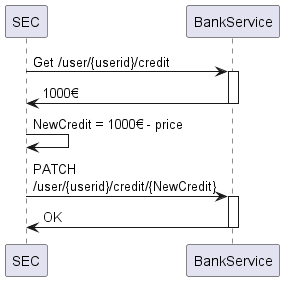
\includegraphics[width=0.3\linewidth]{figures/ChapterVersuchsdurchführung/flawedRemoveMoney-0.png}
	\caption{Sequenzdiagramm für eine Implementierung für \textit{RemoveMoney}, die Dirty Reads verursacht}
	\label{fig:flawed-RemoveMoney}
\end{figure}
\FloatBarrier

\paragraph*{Veränderung von Daten außerhalb des Prozesses} \mbox{} \\
Zusätzlich zu der Abbildung einer fehlerhaften Kommunikation zwischen SEC und Teilnehmerservice können weitere Anomalien auftreten, wenn weitere Prozesse Daten im System verändern. Das können Prozesses außerhalb der Saga sein. Ermöglicht der BankingService beispielsweise das Schließen eines Kundenkontos, treten ebenfalls Isolationsanomalien auf. Ist ein Kunde Bestandteil einer laufenden LLT und schließt während der Ausführung sein Konto, kann es unter Umständen dazu führen, dass die Konsistenz nicht gewährleistet werden kann. Ein weiteres Beispiel ist die Änderung des Preises eines Artikels in dem ArticleService nachdem eine LLT bereits den veralteten Preis validiert hat. Diese Anomalie stellt eine Instanz des Problems des Unrepeatable Reads dar. 

\paragraph*{Verhinderung der Anomalien innerhalb der LLT} \mbox{} \\
Um die Isolationsanomalien auf Ebene der LLT zu vermeiden gibt es keine konkrete Lösung über eine Abstrahierung wie auf Ebene der lokalen Transaktion. Dirty Reads und Lost Updates können bedingt vermieden werden, indem die Kommunikation zwischen dem SEC und dem Teilnehmerservice möglichst wenige Schritte aufweist. Alle Veränderungen, die sich lediglich auf die Daten in einem Teilnehmerservice beziehen, sollten durch den Teilnehmerservice gesteuert werden. Dieser hat die Möglichkeit unter Verwendung von ACID-Transaktionen seine Daten konsistent zu halten, ohne die Isolation zu verletzen.

Isolationsanomalien, die durch andere Prozesse eingeführt werden, können nur verhindert werden, indem das System mit Einschränkungen versehen wird. Eine Einschränkung für das Schließen eines Kontos wäre die Bedingung, dass für den entsprechenden Nutzer keine laufende LLTs existieren. Diese Einschränkungen stellen eine Form der manuellen Implementierung einer Isolationsstufen dar.
